\newpage
\hypertarget{stringRep tex}{}
\subsection{Implementing stringRep}
\texHeader

\vspace{0.5cm}

\begin{itemize}
  
\item[$\blacktriangleright$] Closely following Fig.~\ref{fig:goal_stringRep}, create a nested \texttt{forEach} loop in \texttt{Box.toString()}.
Don't worry about the method invocation just yet, just make sure you return \texttt{this.stringRep}. It should resemble Fig.~\ref{fig:emptyLoops}.

\begin{figure}[htp]
\begin{center}
  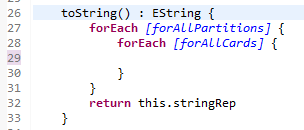
\includegraphics[width=0.5\textwidth]{eclipse_toStringNestedLoops}
  \caption{Control flow for \texttt{toString}}
  \label{fig:emptyLoops}
\end{center}
\end{figure}

\item[$\blacktriangleright$] In order to invoke \texttt{addToStringRep}, we need to introduce a new activity type, our \emph{statement node}. These are
different from patterns as they are able to call methods declared anywhere in the metamodel. This is also their only purpose. They are used strictly for control
flow, to guarantee execution of a task. This special type is declared by surrounding the invocation command with  `\texttt{<>}' tags. Therefore, inside the
second loop, write \texttt{<this.addToStringRepCard>}. The correct \texttt{card} parameter will come from the \texttt{ForAllCards} pattern, which we'll
establish next.

\vspace{0.5cm}

\item[$\blacktriangleright$] The \texttt{toString} activity should now resemble Fig.~\ref{fig:toStringFlow}.

\vspace{0.5cm}

\begin{figure}[htp]
\begin{center}
  \includegraphics[width=0.6\textwidth]{eclipse_boxtoStringFlow}
  \caption{Our first \emph{statement node}}
  \label{fig:toStringFlow}
\end{center}
\end{figure}

\item[$\blacktriangleright$] Despite its complicated appearance, remember - the core idea behind the patterns is to access every item in \texttt{Box}. The
control flow (which we've already established), is where we call a helper function to complete the action. This means both patterns need only create their
object variables and link them together.

\item[$\blacktriangleright$] Complete each patterns as depicted in Fig.~\ref{fig:toStringPatterns}. The second \texttt{partition} is bounded to the one matched
in the first loop, but \texttt{card} is \emph{not} bounded as it doesn't matter how its match is determined.

\vspace{0.5cm}

\begin{figure}[htp]
\begin{center}
  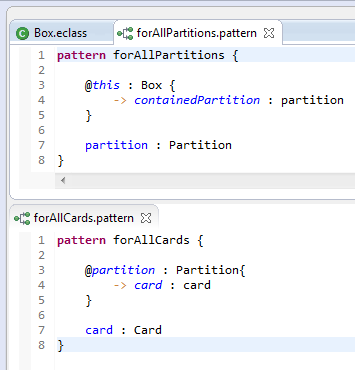
\includegraphics[width=0.6\textwidth]{eclipse_toStringPatterns}
  \caption{Box traversal patterns}
  \label{fig:toStringPatterns}
\end{center}
\end{figure}

\vspace{0.5cm}

\item[$\blacktriangleright$] As crazy at it may seem, that's it!  To see how this SDM is represented visually, check out Fig.~\ref{fig:sdm_tostring_5}.

\end{itemize}
